\chapter{A Guided Tour: What Does a Telescope Actually Record, and Where Is This Book Taking You?}
\label{chap:e00}

\begin{chapteropening}
Tonight, the light from a star has travelled for centuries before finally landing on a mirror. You might imagine that the telescope will store it for you as a photograph, but it will not. What the telescope ultimately writes to disk is neither a continuously undulating electromagnetic wave nor an image that already carries a physical interpretation. It is a long string of labelled detection events: at some instant, in some pixel, in some frequency channel, on some readout channel, another ``click.'' This chapter derives no formulas. It does just two things: first it helps you see clearly what is hidden inside that string of ``clicks,'' and then it unrolls a map of the whole book, telling you where we are going together and why the journey is worth taking.
\end{chapteropening}

\section{What a Telescope Actually Stores the Light As}
\label{sec:e00-event}

Let us first correct a misconception that almost everyone holds. We are used to saying ``the telescope took a picture of the stars,'' as though a painter sat behind the mirror, copying the sky down in real time. The truth is far more modest, and far more interesting: a modern detector (whether one pixel of a CCD, a photomultiplier tube PMT, an avalanche photodiode APD, or a single-photon avalanche diode SPAD) is essentially a ``counter.'' A photon strikes it, it records a ``click''; another strikes, it records another. It does not paint; it counts.

So what a telescope hands us at the lowest level is not an image but an \textbf{event list}: each row corresponds to one photon detection, and each row carries a few labels. Writing the $j$-th detection as one row of data, we have

\begin{equation}
  e_j=\bigl(t_j,\;\bm r_j,\;\nu_j,\;p_j,\;w_j\bigr).
  \label{eq:e00-event}
\end{equation}
\begin{formulaexplain}
\(e_j\) is the row of data for the \(j\)-th photon detection; \(t_j\) is the instant at which it arrived, \(\bm r_j\) is which telescope/pixel it landed on, \(\nu_j\) is which frequency channel it belongs to, \(p_j\) is the polarization or electronics channel, and \(w_j\) is the quality weight of this event. The whole line says: one ``click'' is written down as a row of data ready to be analysed.
\end{formulaexplain}

This expression looks abstract, but every label is in fact very concrete, so let us take them apart one by one:

\begin{itemize}
  \item \(t_j\): the \textbf{arrival time}. This is the time stamp the detector puts on the event; its unit may be seconds or milliseconds, or as fine as nanoseconds (\(\mathrm{ns}=10^{-9}\,\mathrm{s}\)) or even picoseconds (\(\mathrm{ps}=10^{-12}\,\mathrm{s}\)). Do not underestimate this column: later you will see that it is precisely this column that turns ``how photons arrive together'' into measurable physics.
  \item \(\bm r_j\): the \textbf{position label}. It can be the pixel coordinate \((x,y)\) on a CCD, or ``which numbered telescope caught this photon.'' When we talk about interferometry, about two telescopes a hundred metres apart, \(\bm r_j\) is the identifier of that pair of telescopes.
  \item \(\nu_j\): the \textbf{frequency channel}. It records roughly which band of colour this photon belongs to, in units of Hz or simply a channel number. Visible light has frequencies of about \(4\times10^{14}\) to \(8\times10^{14}\,\mathrm{Hz}\); a filter or spectrograph slices this broad band into a number of narrow bins, and \(\nu_j\) is the bin the photon fell into.
  \item \(p_j\): the \textbf{polarization or electronics channel}. It might be ``horizontal or vertical polarization,'' or simply ``which readout circuit it came out of.'' This column is often discarded in traditional data, yet it holds clues to the emission mechanism and the geometry of magnetic fields.
  \item \(w_j\): the \textbf{quality weight}. It is our ``degree of trust'' in this event: did this one strike a bad pixel? Was it right up against the dead time? Might it have come from clouds or background? Rather than crudely throwing away suspect events, we give each one a weight and let the later statistics judge it for themselves. It is a \textbf{dimensionless} number, usually normalized to lie between \(0\) (completely distrusted, equivalent to discarding the event) and \(1\) (fully trusted); intermediate values mean ``accept it at a discount.''
\end{itemize}

Please keep the look of this event list in mind: it is the true protagonist of the whole book. Traditional astronomy is powerful because it knows how to squeeze images, spectra, and light curves out of this list; what this book wants to tell you is that there is still something left over in this list, something that the traditional act of ``taking an average'' happens to wipe away. To see what is left, we must return again and again to the raw ``clicks'' written row by row in Eq.~\eqref{eq:e00-event}.

\section{The Same Batch of Photons Can Be Projected into Many Products}
\label{sec:e00-projection}

The most fascinating thing about the event list is this: \textbf{the same batch of photons can be projected into completely different data products}, just as the same beam of sunlight, passing through window lattices of different shapes, casts different patterns on the floor. Every kind of astronomical ``figure'' we are familiar with is really just one binning of Eq.~\eqref{eq:e00-event} along one of its columns:

\begin{itemize}
  \item Binning by \textbf{position} \(\bm r_j\): pile up the photon counts that landed on the same patch of sky, and you get an \textbf{image}. Where it is bright is where the ``clicks'' are many.
  \item Binning by \textbf{frequency} \(\nu_j\): lay out the photon counts that fell into the same colour bin, and you get a \textbf{spectrum}. The peaks and troughs of the spectral lines are the surplus or deficit of counts in certain channels.
  \item Binning by \textbf{time} \(t_j\): list in order the photon counts in each short slice of time, and you get a \textbf{light curve}. The flickering of a star is the rise and fall of counts in the successive time bins.
  \item Combining by \textbf{polarization channel} \(p_j\): add and subtract the intensities of different polarization channels according to fixed rules, and you get the \textbf{polarization quantities} (the Stokes parameters).
\end{itemize}

There is one key sentence worth repeating three times: \textbf{every projection preserves part of the information while discarding another part}. When, in order to draw an image, you ``compress'' the millions of photons in a pixel into a single brightness number, you do get ``how bright it is here,'' but you forever erase ``whether those millions of photons like to arrive together in crowds.'' When, in order to draw a light curve, you compress each millisecond's photons into a single count, you can no longer tell whether the photons in that same millisecond fell sparsely and independently, or clustered into a clump within a few microseconds.

This is the move the book will make again and again: \textbf{before you project, stop and ask: what am I about to throw away?} For some astrophysical questions, projecting into an image is enough; but the angular diameter of a star, the structure at the edge of a black hole, the signatures of certain new physics: these hide precisely in the joint relationships between photon and photon that get ``averaged away.'' Once you average first, you can never fish them back. Figure~\ref{fig:e00-event-map} draws this as a map: at the centre is the same event list, and radiating out on all sides are the various products it can become.

\begin{figure}[tbp]
\centering
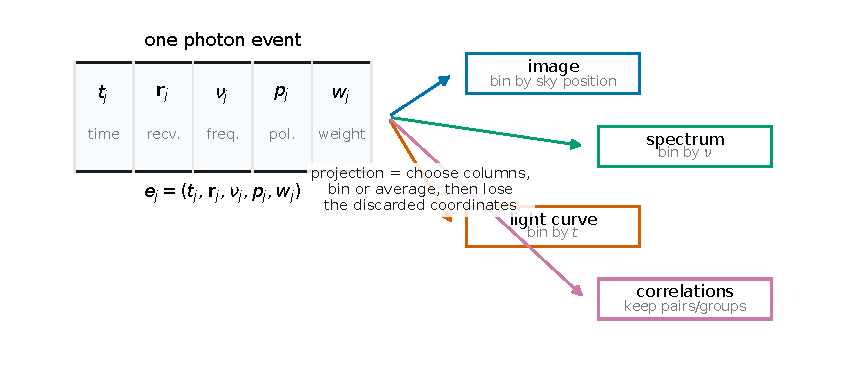
\includegraphics[width=0.9\linewidth]{figures/generated/chapter_01/ch01_event_table_map.pdf}
\caption{The same photon event list can be projected into many kinds of data products. Binning along position gives an image, binning along frequency gives a spectrum, binning along time gives a light curve, and combining across polarization channels gives the polarization quantities. Every projection preserves part of the information and discards part; relationships such as ``how photons arrive together in pairs'' become visible only when one returns to the raw event list.}
\label{fig:e00-event-map}
\end{figure}

\section{Light Speaks Two Languages: Wave, and Count}
\label{sec:e00-two-languages}

To read what has been ``thrown away'' in the event list, you must first accept something that physicists argued about for a century: \textbf{light speaks two languages at once}, and the two languages describe one and the same thing.

The first is the \textbf{language of the wave}. Within a sufficiently narrow band of colour, light can be regarded as a train of oscillating electromagnetic waves: what is really trembling is the electric field, which has an amplitude, a phase, and interferes. Superpose two beams: crest on crest is brighter, crest on trough is dimmer: this is constructive and destructive interference. Phase, interference, fringes are the keywords of this language. The electric field of visible light must oscillate hundreds of trillions of times per second, one period lasting only a few femtoseconds (\(\mathrm{fs}=10^{-15}\,\mathrm{s}\)), too fast for any ordinary detector to keep up with; and so the detector cannot see the positive and negative swings of the field, and can only smooth these rapid oscillations over its own response time, leaving in the end only the energy.

The second is the \textbf{language of counting}. What the detector leaves behind is a set of discrete ``clicks,'' each one the tap of a single photon. Since these are independent random taps one after another, the count must inevitably carry fluctuations: even if the source brightness, the telescope, and the detector all hold perfectly still, the number of photons you count each millisecond will still jitter up and down. This inborn jitter is called \textbf{shot noise} (also called Poisson noise); it is not a flaw of the instrument, but the inevitable shadow of the fact that ``light really is counted out one grain at a time.''

These two languages sound like polar opposites (one speaks of continuous waves and phase, the other of discrete taps and probability), but the whole charm of quantum astronomy lies in the fact that they are two faces of the same coin, and can both be read out of the \textbf{event list}. Here I will only give a preview, planting three threads:

\begin{itemize}
  \item The language of the wave (electric field, complex amplitude, phase, interference) will be formally taken up in Chapter~\ref{chap:e01}, where we will write the electric field as a ``rotating arrow''; Chapter~\ref{chap:e02} then extends it through Fourier analysis, making clear the notions of bandwidth and coherence time, that is, ``how long can this arrow remember its own phase.''
  \item The language of counting (probability, Poisson statistics, shot noise) will be worked out in Chapter~\ref{chap:e03}, where we go from the most naive picture of ``slice time into many little cells'' all the way to the Poisson distribution, computing the fluctuation of the ``clicks'' as a predictable number.
  \item With these two languages in hand, we must first make the ``photon'' itself rigorous: Chapter~\ref{chap:e04} supplies the ladder operators of quantum mechanics and the harmonic oscillator, and Chapter~\ref{chap:e05} uses them to give the quantization of light. Only this is the thread and needle that truly sews ``wave'' and ``count'' into one and the same mathematics.
  \item And the bridge that welds these two languages fully together, that turns ``coherence of the wave'' directly into ``correlation of the counts,'' intensity interferometry and the Hanbury Brown--Twiss (HBT) effect, belongs to Part 2 of the book, ``Coherence and Correlation.'' It is only there, in chapters even later than the quantization of light, that it is formally erected.
\end{itemize}

In other words, the suspense this chapter has planted (``how a single batch of photons arrives together, and what is hidden in that'') can only be fully explained when the two languages are joined. Chapters~\ref{chap:e01} through~\ref{chap:e05} first sharpen each of the two languages on its own and make the ``photon'' rigorous; the HBT correlation that truly brings the two together is left for the later part on ``Coherence and Correlation'' to reel in.

\section{The Promise of This Book: Why It Is Worth Learning This ``Quantum'' Language}
\label{sec:e00-promise}

You might ask: traditional astronomy can already deliver images, spectra, light curves, and polarization, and gets along just fine, so why go to the trouble of learning this ``quantum'' language of returning to the event list and watching how photons arrive together? Because it can do some things that traditional methods \textbf{cannot do in principle}. This is not treating ``quantum'' as a gimmick, but a matter of real scientific returns.

\textbf{Measuring the true size of a star.} Stars are so far away that in a telescope they are almost all just a point. Their angular diameters are as small as the milliarcsecond (mas, i.e.\ \(10^{-3}\) arcsecond) or even the microarcsecond. How small is that? \(1\,\mathrm{mas}\approx4.85\times10^{-9}\,\mathrm{rad}\); to make a coin about \(2.5\,\mathrm{cm}\) in diameter subtend such a small angle, you would have to place it about five thousand kilometres away, roughly half the distance from Beijing to London; and a microarcsecond is another thousand times smaller. An ordinary telescope, limited by the diffraction limit, simply cannot resolve such fine angular structure, but intensity interferometry can correlate the photon counts of two telescopes a hundred metres or a kilometre apart, and from ``how synchronized the fluctuations of the two telescopes are'' infer this angular diameter. A star is no longer a point, but acquires a measurable disk, a shape flattened by rotation, and limb darkening at its edge.

\textbf{Approaching the edges of black holes and compact objects.} Longer baselines and higher time resolution can in principle push this method toward smaller angular scales, to constrain accretion disks, stellar winds, and even the structure around compact objects.

\textbf{Putting new physics on a leash.} The extremely precise measurement of photon arrival times and correlations can also be used to test ideas beyond the Standard Model. Any question that can be written as ``an estimable quantity in the event list $+$ an honest error budget $+$ a null test'' may become a genuinely executable observing program.

These are not idle words on paper. Please remember three real names, which will recur throughout the book:

\begin{itemize}
  \item \textbf{Narrabri}: in the 1960s, the stellar intensity interferometer at Narrabri, Australia, used two large reflectors that could slide along a track to systematically measure, for the first time, the angular diameters of dozens of bright stars. This is the starting point of the craft.
  \item \textbf{VERITAS} and \textbf{MAGIC}: today, large Cherenkov telescope arrays (each more than ten metres in aperture) originally built to catch high-energy gamma rays have been cleverly repurposed as optical intensity interferometers, measuring the sub-milliarcsecond angular diameters of bright stars to a precision of a few percent. A method that lay dormant for years because its signal was too weak has, thanks to large mirrors, fast electronics, and digital correlators, come back to life.
\end{itemize}

Figure~\ref{fig:e00-science-map} places these science goals on the same map: read horizontally it is ``how close to conventional observation,'' read vertically it is ``how much new information beyond the reach of traditional methods.'' The angular diameters of bright stars are already within arm's reach, while farther out lie goals of extremely high value that demand more engineering breakthroughs, such as supernova distance measurement and the quantum-network telescope. This figure is the territory the book wishes to invite you to explore together.

\begin{figure}[tbp]
\centering
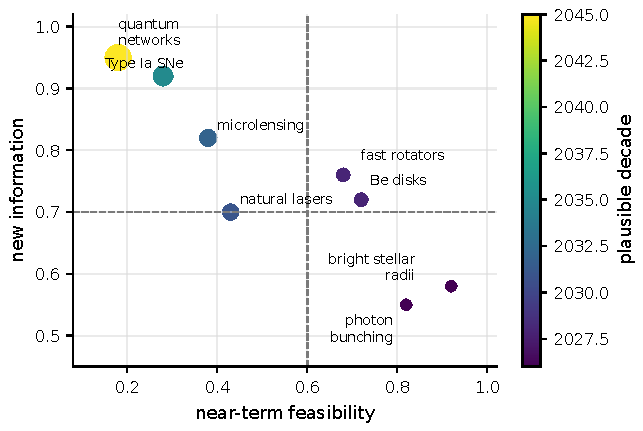
\includegraphics[width=0.8\linewidth]{figures/generated/chapter_02/ch02_science_case_map.pdf}
\caption{A map of the first-generation science questions of quantum astronomy: the horizontal axis roughly indicates distance from conventional observation, and the vertical axis indicates the amount of information gained relative to traditional methods. The angular diameters of bright stars and stellar photon bunching are already close to present capability; fast rotators, stellar disks, and natural masers are near-term extensions; supernova angular-distance measurement and the quantum-network telescope are of the highest value but require engineering breakthroughs such as longer baselines, fast triggering, or quantum links.}
\label{fig:e00-science-map}
\end{figure}

\section{A Map of the Whole Book: The Seven Stops We Will Travel Together}
\label{sec:e00-map}

Finally, let us unroll the whole map. The book is divided into seven parts (Part 0 through Part 6), like a construction route that builds from the foundation all the way up to the roof. You need not read it all in one go, but you had best know which storey each stop is building:

\begin{itemize}
  \item \textbf{Part 0: Foundations and languages.} These are the very chapters you are reading. We hone two tools: the language of the wave (electric field, complex amplitude, phase, interference) and the language of counting (Poisson statistics, shot noise, order-of-magnitude estimation). The goal is that whenever you meet a formula, you first see the physical picture behind it.
  \item \textbf{Part 1: The quantum description of light.} Making the word ``photon'' rigorous: from the quantization of the electric field to the coherent state, the thermal state, and the number state, understanding why laser-like coherent light and star-like thermal light differ so profoundly in ``how their photons arrive together.''
  \item \textbf{Part 2: Coherence and correlation.} The heart of the book. First-order coherence \(g^{(1)}\) (interference, visibility) and second-order coherence \(g^{(2)}\) (photon bunching, intensity correlation) make their entrance here, the Siegert relation welds the two together, and the HBT effect turns from a ``bizarre phenomenon'' into ``computable physics.''
  \item \textbf{Part 3: From correlation to imaging.} The van Cittert--Zernike theorem tells us how the brightness distribution of the sky is encoded into the spatial coherence; and so ``the correlation of two telescopes'' is translated into ``the angular diameter of a star,'' and the principle of intensity-interferometric imaging closes the loop here.
  \item \textbf{Part 4: The limits of measurement.} Introducing Fisher information and the Cramér--Rao lower bound to answer an honest question: given so many photons and so long an integration time, how precisely can we \textbf{at best} measure the angular diameter? The noise budget is laid on the table here.
  \item \textbf{Part 5: Real instruments and observations.} The atmosphere, detector jitter, dead time, background, clock synchronization, the \(u,v\) coverage of multiple telescopes: bringing the ideal formulas down into the mud of real systems such as Narrabri, VERITAS, and MAGIC.
  \item \textbf{Part 6: Frontiers and outlook.} Frequency and polarization correlations, natural masers, microlensing, quantum-enhanced measurement, and the quantum-network telescope, pushing the boundary of the map toward regions still under exploration.
\end{itemize}

\textbf{How should this book be used?} If you are an undergraduate, please read in order, and treat every formula annotated with a small \verb|formulaexplain| note as a ``prompt card'': first read the physical picture in the main text, then go back and check the unit and meaning of every symbol; when you meet a derivation, do not skip steps: the book has already written out every intermediate step, and all you need to do is walk through it once. If you already have a background, you may jump straight to \(g^{(2)}\) in Part 2 and the information limits in Part 4, which is where the book's information density is highest. However you enter, remember to glance back at this map from time to time and ask yourself: \emph{which stop am I standing at now, and which storey is the tool in my hand meant to build?}

\section{Chapter Summary}
\label{sec:e00-summary}

\begin{itemize}
  \item A telescope stores neither the wave nor an image, but a labelled \textbf{photon event list}, each row being \(e_j=(t_j,\bm r_j,\nu_j,p_j,w_j)\): time, position, frequency channel, polarization/electronics channel, and quality weight.
  \item Images, spectra, light curves, and polarization quantities are all \textbf{projections} of this list along different columns; every projection preserves part of the information and discards part, while ``how photons arrive together in pairs'' is visible only in the raw event list.
  \item Light speaks both the \textbf{language of the wave} (electric field, phase, interference) and the \textbf{language of counting} (taps, Poisson noise); Chapters~\ref{chap:e01} through~\ref{chap:e03} sharpen each of these two languages (wave and coherence time in Chapters~\ref{chap:e01} and~\ref{chap:e02}, Poisson and shot noise in Chapter~\ref{chap:e03}), and Chapters~\ref{chap:e04} and~\ref{chap:e05} then make the ``photon'' rigorous; the HBT correlation that truly brings the two together is left for Part 2, ``Coherence and Correlation,'' to reel in.
  \item The reward for learning this language is tangible: \textbf{stellar angular diameters} at the milliarcsecond and even microarcsecond level, the edges of compact objects, and constraints on new physics; Narrabri, VERITAS, and MAGIC have already turned it from concept into measurement.
\end{itemize}

\medskip
\noindent\textbf{Questions to Ponder.}
\begin{itemize}
  \item If you were allowed to keep only \textbf{one column} of the event list, which column would you keep? To answer ``how big is the star,'' which column can least afford to be lost?
  \item For the same stretch of observation, what does compressing it into an image throw away and keep, and what does compressing it into a light curve throw away and keep? Is there any kind of information that neither projection can retain?
  \item ``Shot noise'' is not a defect of the instrument but the inevitable consequence of light being counted one grain at a time. So if you double the integration time, roughly what fraction of its original value does the relative fluctuation become? (Hint: think about \(1/\sqrt{\mu}\).)
\end{itemize}
